\documentclass{article}
\usepackage[utf8]{inputenc}

% Language setting
% Replace `english' with e.g. `spanish' to change the document language
\usepackage[english]{babel}
\usepackage{float}
\usepackage{multicol}

% Set page size and margins
% Replace `letterpaper' with `a4paper' for UK/EU standard size
\usepackage[letterpaper,top=2cm,bottom=2cm,left=3cm,right=3cm,marginparwidth=1.75cm]{geometry}

% Useful packages
\usepackage{amsmath}
\usepackage{graphicx}
\usepackage{wrapfig}
\usepackage{svg}

\usepackage[colorlinks=true, allcolors=blue]{hyperref}

\title{OranJam}
\author{Lelio Casale, Marco Furio Colombo, Marco Muraro, Matteo Pettenò }
\date{10582124, 10537094, 10866647, 10868930}

\begin{document}

\maketitle

\begin{abstract}
Sound Synthesis refers to the possibility of generating sound from scratch, using electronic hardwares or softwares. The sound is produced according to some chosen parameters in function of the result that the musician wants to get.
\\A synthesizer is an electronic musical instrument which is able to generate different signals and then manipulate them to achieve a specific sound as a final result.
\\The Hammond Organ, released in 1935, was the first electronic instrument to become popular within the music industry and today it’s considered a precursor to modern synths. The very first synthesizer was RCA’s MARK II Sound Synthesizer, released in 1957. This instrument was able to read punch cards that controlled a synthesizer made of 750 vacuum tubes. Nevertheless, the dawn of modern synthesizers is considered 1964 to around the mid-70s. As a matter of facts, in those years engineer Robert Moog brought a real revolution among electronic instruments. This revolution started with the Moog synthesizer which was released in 1964.
Today, different synthesis techniques can be exploited to generate different kinds of sounds. The most common ones are \textbf{subtractive synthesis}, \textbf{additive synthesis} and \textbf{frequency modulation synthesis} (FM synthesis).
\\The project presented in the following paper is the implementation of a subtractive synthesizer and its interface meant to allow for the user to control a different kind of parameters shaping the generated sound.

\end{abstract}

\section{Introduction}

\subsection{Basic Principles of Subtractive Synthesis}

Subtractive synthesis technique comes from the idea of generating a sound starting from an existing signal whose partials are attenuated by a filter to modify its timbre. The starting sound is often the result of different signals that are mixed together. Generally, the musician starts from sounds that are very rich in harmonics and exploits different kinds of filtering and tools that shape the spectrum of sound.
\\Subtractive Synthesizers are sound signals generators which can be controlled by a musician through a control panel, a keyboard or other devices. These synthesizers are equipped with one or more oscillators, also called VCO (Voltage Controlled Oscillator, with regard to analog synthesizers), that generate standard waveforms such as sine wave, saw tooth wave, square wave and triangle wave. Furthermore, a noise generator could be available to produce white noise or pink noise to obtain more interesting sounds. These sound waves are mixed together to get the starting signal to be filtered later. Sometimes frequencies are slightly different so that it's possible to obtain beating effect and more interesting and complex sounds.
\\Several kinds of filters could be available to be used for modifying the timbre of the sound according to the final result that the user wants to obtain: low-pass filter, high-pass filter, band-pass filter, band-reject filter, shelving filters (high, low, peak/notch shelving filters).
\\Normally a hardware synthesizer is provided with a keyboard or it can be connected to an external MIDI keyboard so that the oscillators are triggered every time a Note On MIDI message is sent by the keyboard to the synth itself. The generated sound is then modified in its amplitude by a so-called VCA (Voltage Controlled Amplitude) which defines attack, decay, release and sustain envelope phases. Subsequently, one or more filters are applied on the signal. In some cases, the cut-off frequency depends on the fundamental frequency of the note that has been played. This parameter is called key follow because the cut-off frequency follows the frequency related to the key that has been pressed on the MIDI keyboard.
\begin{figure}[H]
\centering
 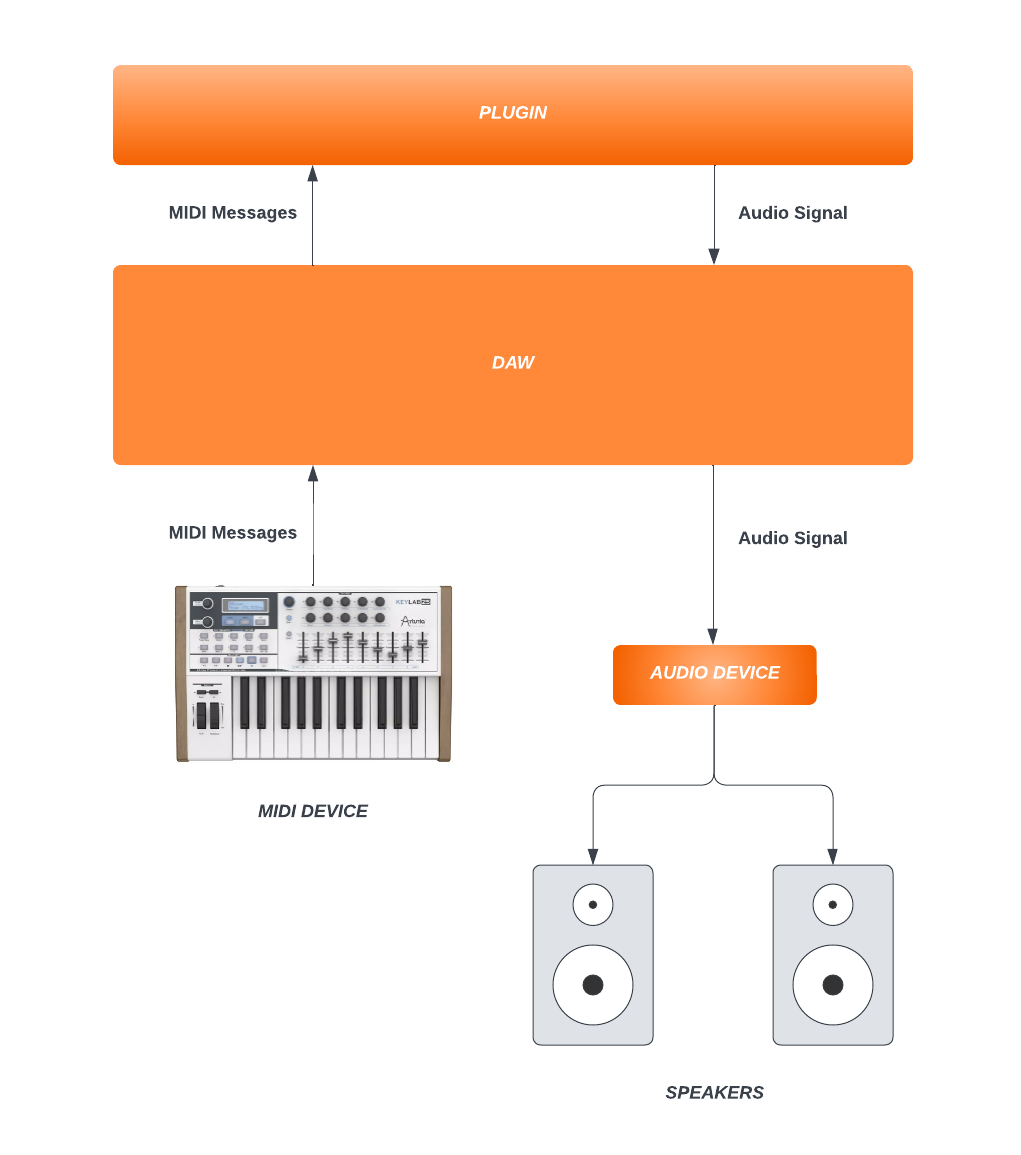
\includegraphics[width=0.8\textwidth]{DSP System Scheme.png}
  \caption{Scheme of interaction between MIDI inputs, DAW, Plugin and Audio Device.}
\end{figure}
The filter could also have its own free-standing envelope to be applied on cutoff frequency (VCF: Voltage Controlled Filter). Of course, Q factor could be controlled in the same way with a different envelope.
As said before, filter’s parameters can be controlled by the frequency or the amplitude of the note that has been played. Another control tool that could be present is the LFO (Low Frequency Oscillator) that provides the user with the possibility of producing a sort of vibrato effect on the final sound.
\\Subtractive synthesis allows the musician to play very interesting and bright sounds at a low computational cost. The user can easily choose the starting waveform, the type of filter to be applied and its parameters such as cutoff frequency and Q factor. Few and simple controls to generate complex and wonderful sounds.


\subsection{Purposes}

The project aims to develop an instrument plugin which implements a subtractive synthesizer. The software was implemented in C++ language with the aid of JUCE framework, a very powerful multi-platform and cross-standard library which supports different operating systems (MacOS, Windows, Linux) and plugin standards available on the market today (VST, VST3, Audio Unit, Audio Unit V3, RTAS, AAX).
The synth should provide the musician with the following primary features:
\begin{itemize}
    \item different sound \textbf{generators}: a white noise generator and two or more \textbf{oscillators}. Oscillators can produce soundwaves of different nature, such as sine wave, saw tooth wave and square wave.
    \item \textbf{envelope} control. The user should be able to change attack, decay, sustain and release parameters of the starting sound that has been obtained by mixing together signals coming from noise generator and oscillators bank.
    \item different kinds of \textbf{filters} to be used for modifying the timbre of the sound according to the final result that the user wants to obtain. Three types of filters should be available: low-pass, high-pass and peak filter. For each of them the musician can control cut-off frequency and resonance. Moreover, it should be possible to control a gain parameter for the peak filter.
    \item an \textbf{LFO} (Low Frequency Oscillator) to be applied as a gain control on the starting signal for creating vibrato effect.
    \item a \textbf{Graphical User Interface (GUI)} to enable the user to control all the parameters specified above.
\end{itemize}
\section{Implementation}

\subsection{Software Architecture}

The file \textit{SubtractiveSynth.jucer} allows the user to run the software and export it in an external IDE in order to actually build the code. The alternative building method is trought the usage of CMake and the needed files are included in the project as well.

\begin{wrapfigure}{l}{0.55\textwidth}
{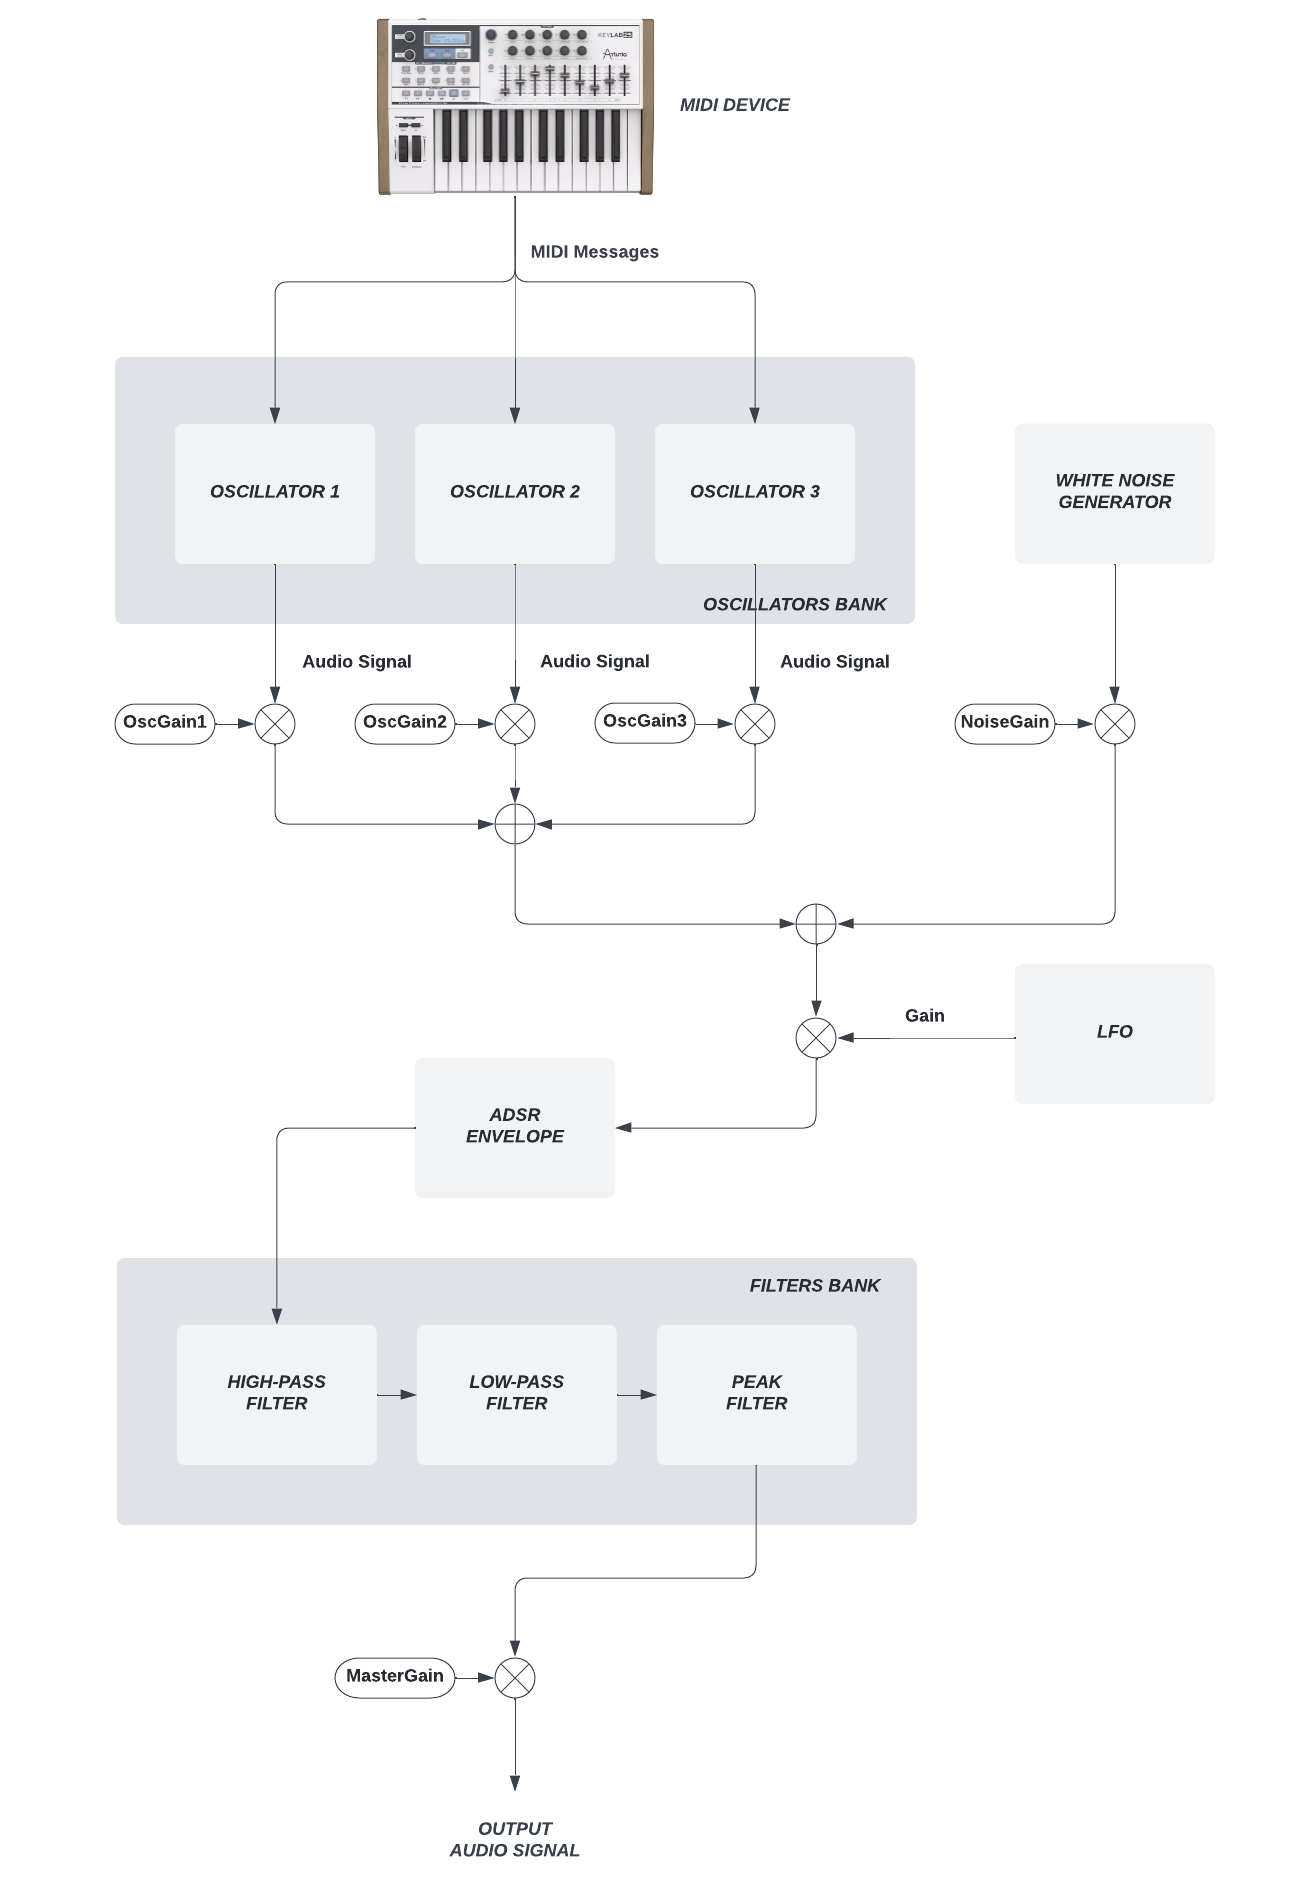
\includegraphics[width=9.35cm]{Signal Flow Diagram.png}}\par
    \caption{Signal Flow Diagram.}
\end{wrapfigure}

The software architecture is designed to be as modular as possible. Exploiting the Object-Oriented nature of the C++ programming language, the software is divided in many classes: each one implements a specific functionality of the plugin. The namespaces \textbf{\textit{$\sim$Generators}}, \textbf{\textit{$\sim$Oscillators}} and \textbf{\textit{$\sim$Filters}} are external modules, included in the Modules package.
\\The class \textbf{\textit{$\sim$PluginProcessor}} creates the plugin and instantiates the oscillator voices needed for the Generators. It also prepares the parameters and sets up the graphical features of the plugin.
\\The class \textbf{\textit{$\sim$SubtractiveSynth}} contains the main core of the plugin. The method \textbf{\textit{prepareToPlay()}} prepares all the parts of the plugin (oscillators, filters, LFO, gain knobs) to be ready to process the signal. The goal of the \textbf{\textit{update()}} method is to interact with the GUI: thanks to this implementation, every time a knob or slider is changed by the user in the graphical part, the corresponding value is sent to the processor through the \textbf{\textit{$\sim$AudioProcessorValueTreeState}} and the parameters are updated in real time to provide the desired signal processing. 
The method \textbf{\textit{renderNextBlock()}} implements the effective signal flow chain: first step are the three oscillators. On the resulting signal a white noise and then the LFO and the envelope are applied, then the high-pass, low-pass and peak filters in sequence, and finally the master gain (\textit{Figure 2}).  
\\The class \textbf{\textit{$\sim$ParametersManager}} initializes all the parameters of the subtractive synthesizer and sets all their value ranges thanks to the \textbf{\textit{$\sim$juce::NormalisableRange}} object.
\\The namespace \textbf{\textit{$\sim$Oscillators}}, thanks to its subclass \textbf{\textit{$\sim$MultiWavesOscillator}}, generates the sinusoidal, square and saw original waves.
\\The class \textbf{\textit{$\sim$Envelope}}, placed inside \textbf{\textit{$\sim$Generators}}, implements the ADSR in the signal flow, and \textbf{\textit{$\sim$WhiteNoise}} provides all the functionalities that are needed to generate the white noise, added afterwards to the waveforms.
\\The namespace \textbf{\textit{$\sim$Filters}} has everything it needs to implement the filters, importing the \textbf{\textit{$\sim$HPFilter}}, \textbf{\textit{$\sim$LPFilter}} and \textbf{\textit{$\sim$PeakFilter}} classes.
\\The package \textit{foleys\_gui\_magic} is imported in order to provide all the functionalities of the graphical user interface.

\subsection{Audio Processing}

\subsubsection{Oscillators}
The implemented synthesizer features an oscillators bank which consists of three different oscillators. The software provides the musician with the possibility of setting different waveforms (sine wave, saw tooth wave and square wave) according to the desired sound. 
For this purpose, an external module was implemented. As a matter of facts, the single oscillator is modeled through the \textbf{\textit{$\sim$Oscillators::MultiWavesOscillator}} class. 
\\\textbf{\textit{MultiWavesOscillator::prepare()}} calls prepare method of \textbf{\textit{$\sim$juce::dsp::Oscillator}} class which takes a \textbf{\textit{$\sim$juce::dsp::ProcessSpec}} object as an input. This method allows to set sampleRate, samplesPerBlock and outputChannels parameters so that the oscillator is ready to play. \textbf{\textit{MultiWavesOscillator::prepare()}} is called in \textbf{\textit{SynthVoice::prepareToPlay()}} method where a processSpec object is instantiated. Then, a for cycle allows to call prepare method on each oscillator instance.
\\\textbf{\textit{MultiWavesOscillator::process()}} is called within \textbf{\textit{renderNextBlock()}} of \textbf{\textit{$\sim$SynthVoice}} class. This method, on its turn, calls \textbf{\textit{Oscillator::process()}} method of juce dsp module which processes the input and output buffers that are supplied in the processing context that is passed as an input. 
\\Another very important method within this class is \textbf{\textit{setWaveType()}} which allows to set the chosen waveform for the single oscillator. The musician can change wave type directly through the graphical user interface, which was implemented using the \textit{foleys\_gui\_magic} module.
Then, \textbf{\textit{updateParameters()}} method enables updating of waveType, frequency and gain of the single oscillator. This method is called within \textbf{\textit{SynthVoice::update()}} that updates all the processing parameters.

\subsubsection{Generators}
Moreover, the synth features a \textbf{white noise generator}, an \textbf{ADSR envelope} and a \textbf{LFO}. For this reason, an external module, called \textbf{\textit{$\sim$Generators}}, was implemented including \textbf{\textit{$\sim$WhiteNoise}}, \textbf{\textit{$\sim$Envelope}} and \textbf{\textit{$\sim$LFO}} classes.
\textbf{\textit{$\sim$Generators::WhiteNoise}} class models a white noise generator. 
\begin{itemize}
    \item \textbf{\textit{process()}} method is called within \textbf{\textit{SynthVoice::renderNextBlock()}} method and exploits \textbf{\textit{$\sim$juce::Random}} class to generate random-valued samples to be inserted within the audio buffer that is passed as an input.
    \item \textbf{\textit{updateParameters()}} method simply updates the gain that is set by the musician through the GUI.
\end{itemize}
\textbf{\textit{$\sim$Generators::Envelope}} class implements the envelope which is provided by the synthesizer. It inherits from \textbf{\textit{$\sim$juce::ADSR}} class that needs a \textbf{\textit{$\sim$juce::ADSR::Parameters}} object as a member. 
\begin{itemize}
    \item \textbf{\textit{prepare()}} method is called within \textbf{\textit{prepareToPlay()}} of \textbf{\textit{$\sim$SynthVoice}} class. This method resets the envelope to an idle state and then sets the sampleRate.
    \item \textbf{\textit{updateParameters()}} simply updates attack, decay, sustain and release parameters. Then, \textbf{\textit{setParameters()}} of \textbf{\textit{$\sim$juce::ADSR}} class is called so that the \textbf{\textit{$\sim$juce::ADSR::Parameters}} object is updated as well. Before updating ADSR parameters, \textbf{\textit{Generators::Envelope::prepare()}} method must have been called. As a matter of facts, \textbf{\textit{setParameters()}} needs to be called after the sampleRate is updated, otherwise the processed values could be incorrect.
    \item \textbf{\textit{process()}} is called within \textbf{\textit{$\sim$SynthVoice::renderNextBlock}} and, on its turn, calls \textbf{\textit{applyEnvelopeToBuffer()}} of \textbf{\textit{$\sim$juce::ADSR}} class so that the envelope is applied to the audioBuffer that is passed as an input.
\end{itemize}
\textbf{\textit{$\sim$Generators::LFO}} class models a Low Frequency Oscillator (LFO). The LFO is implemented through a \textbf{\textit{$\sim$juce::dsp::Oscillator}} object. Similarly to other classes described before, \textbf{\textit{prepare()}} sets the sampleRate, samplesPerBlock and outputChannels of the oscillator. Then, \textbf{\textit{process()}} method computes the LFO sample by sample. Subsequently, the LFO is applied to the whole input audio buffer as a gain. \textbf{\textit{updateParameters()}} enables to initialize the oscillator and set its frequency and amount.

\subsubsection{Filters}

Another important part of the synthesizer is the \textbf{filters} block, which provides the user with the possibility of cutting some frequencies and amplifying others. This is made thanks to the three filters implemented: an \textbf{high-pass}, a \textbf{low-pass} and a \textbf{peak} filter. All these filters are infinite impulse response filters and are implemented in the same way through the \textbf{\textit{makeLowPass()}}, \textbf{\textit{makeHighPass()}} or \textbf{\textit{makePeakFilter()}} methods provided by juce in the \textbf{\textit{$\sim$IIR::Coefficients}} class included in the dsp module. The choice of infinite impulse response filters was made in order to maintain the signal as much analog as possible: IIR filters derive from analog, while FIR filters have no analog history. 
\\The high-pass and low-pass filters have two parameters: the cutoff frequency and a resonance value, also called Q factor. On the other hand, the peak filter has three parameters: the peak frequency, the resonance or Q factor value and the gain which the filter provides the peak frequency with.
\\Each filter type has its own juce class with three main methods: 
\begin{itemize}
    \item the \textbf{\textit{prepare()}} method is called in the \textbf{\textit{preparetoPlay()}} method of the \textbf{\textit{$\sim$SubtractiveSynth}} class and initializes the filter to be ready for its functionalities.
    \item the \textbf{\textit{process()}} method is called in the \textbf{\textit{renderNextBlock()}} method of the \textbf{\textit{$\sim$SubtractiveSynth}} class and implements the signal filtering in the process chain.
    \item the \textbf{\textit{updateParameters()}} method is called in the \textbf{\textit{update()}} method of the \textbf{\textit{$\sim$SubtractiveSynth}} class and sends the commands from the graphical user interface to the plugin processor.
\end{itemize}

\section{Graphical User Interface (GUI)}
The \textit{juce} framework offers the chance to create a custom Graphical User Interface (GUI) that implements and connects all parameters of interest in a designed component called the \textit{PluginEditor} basically from scratch. However, during the preliminary phase of design of the synthesizer, we found an external library called \textit{foleys\_gui\_magic} \href{https://github.com/ffAudio/foleys_gui_magic}{(GitHub repository)}, that would allow us to have a better workflow and ultimately a more pleasing GUI. For this reason, we decided  to use it.

\subsection{foleys\_gui\_magic}
We can essentially break what this library does down to two aspects: creates a CSS cascading stylesheet in an \textit{xml} file to define rules for the appearance of the GUI and fetches the parameters from the \textit{\textbf{$\sim$AudioProcessorValueTreeState}} matching them with the GUI elements of choice. This allows the \textit{\textbf{$\sim$PluginEditor}} to be substituted with the \textit{\textbf{$\sim$MagicPluginEditor}}, generated by the library itself.
\\
Besides allowing us to avoid writing a lot of boilerplate code and to not reinvent the wheel when making the interface, \textit{foleys\_gui\_magic} helped us with our workflow. It made possible preparing all the components and linking them to the interface before actually creating one and therefore we were able to create an effective graphical design when we already had a clear view of all the components we prepared without issues. The \textit{xml} file that defines the rules that model the layout has also proven really useful, giving an alternative method to modify views in a CSS-like fashion, granting additional flexibility to the framework.

The inclusion of \textit{foleys\_gui\_magic} is just as simple as the one of any other module and can be done both using the \textbf{projucer} app or \textbf{CMake}. Of course in the deployed product none of that is necessary, since the inclusion has already happened in build. Once the \textit{foleys\_gui\_magic} is added to the project, the usage is rather simple: it offers both a graphical way of modifying the plugin layout and the said \textit{xml}.
\\
Understanding how this module works has proven to be quite a challenge, due to the minimal documentation, but was quite interesting for us in the end. Its work pattern is to create a \textbf{“Magic”} extension of the \textit{juce} components of interest, expanding their functionalities or entirely substituting them. What allows parameter refreshing is the \textit{\textbf{$\sim$MagicProcessorState}}, which is linked to the \textit{\textbf{$\sim$AudioProcessorValueTreeState}} and listens to its changes, feeding them to the \textit{\textbf{$\sim$MagicProcessor}}. Said processor is created by a dedicated builder using the \textit{xml}-specified layout and the designed connections, such as the ones for spectral visualization. 
\vspace{20pt}
\begin{figure}[H]
\centering
  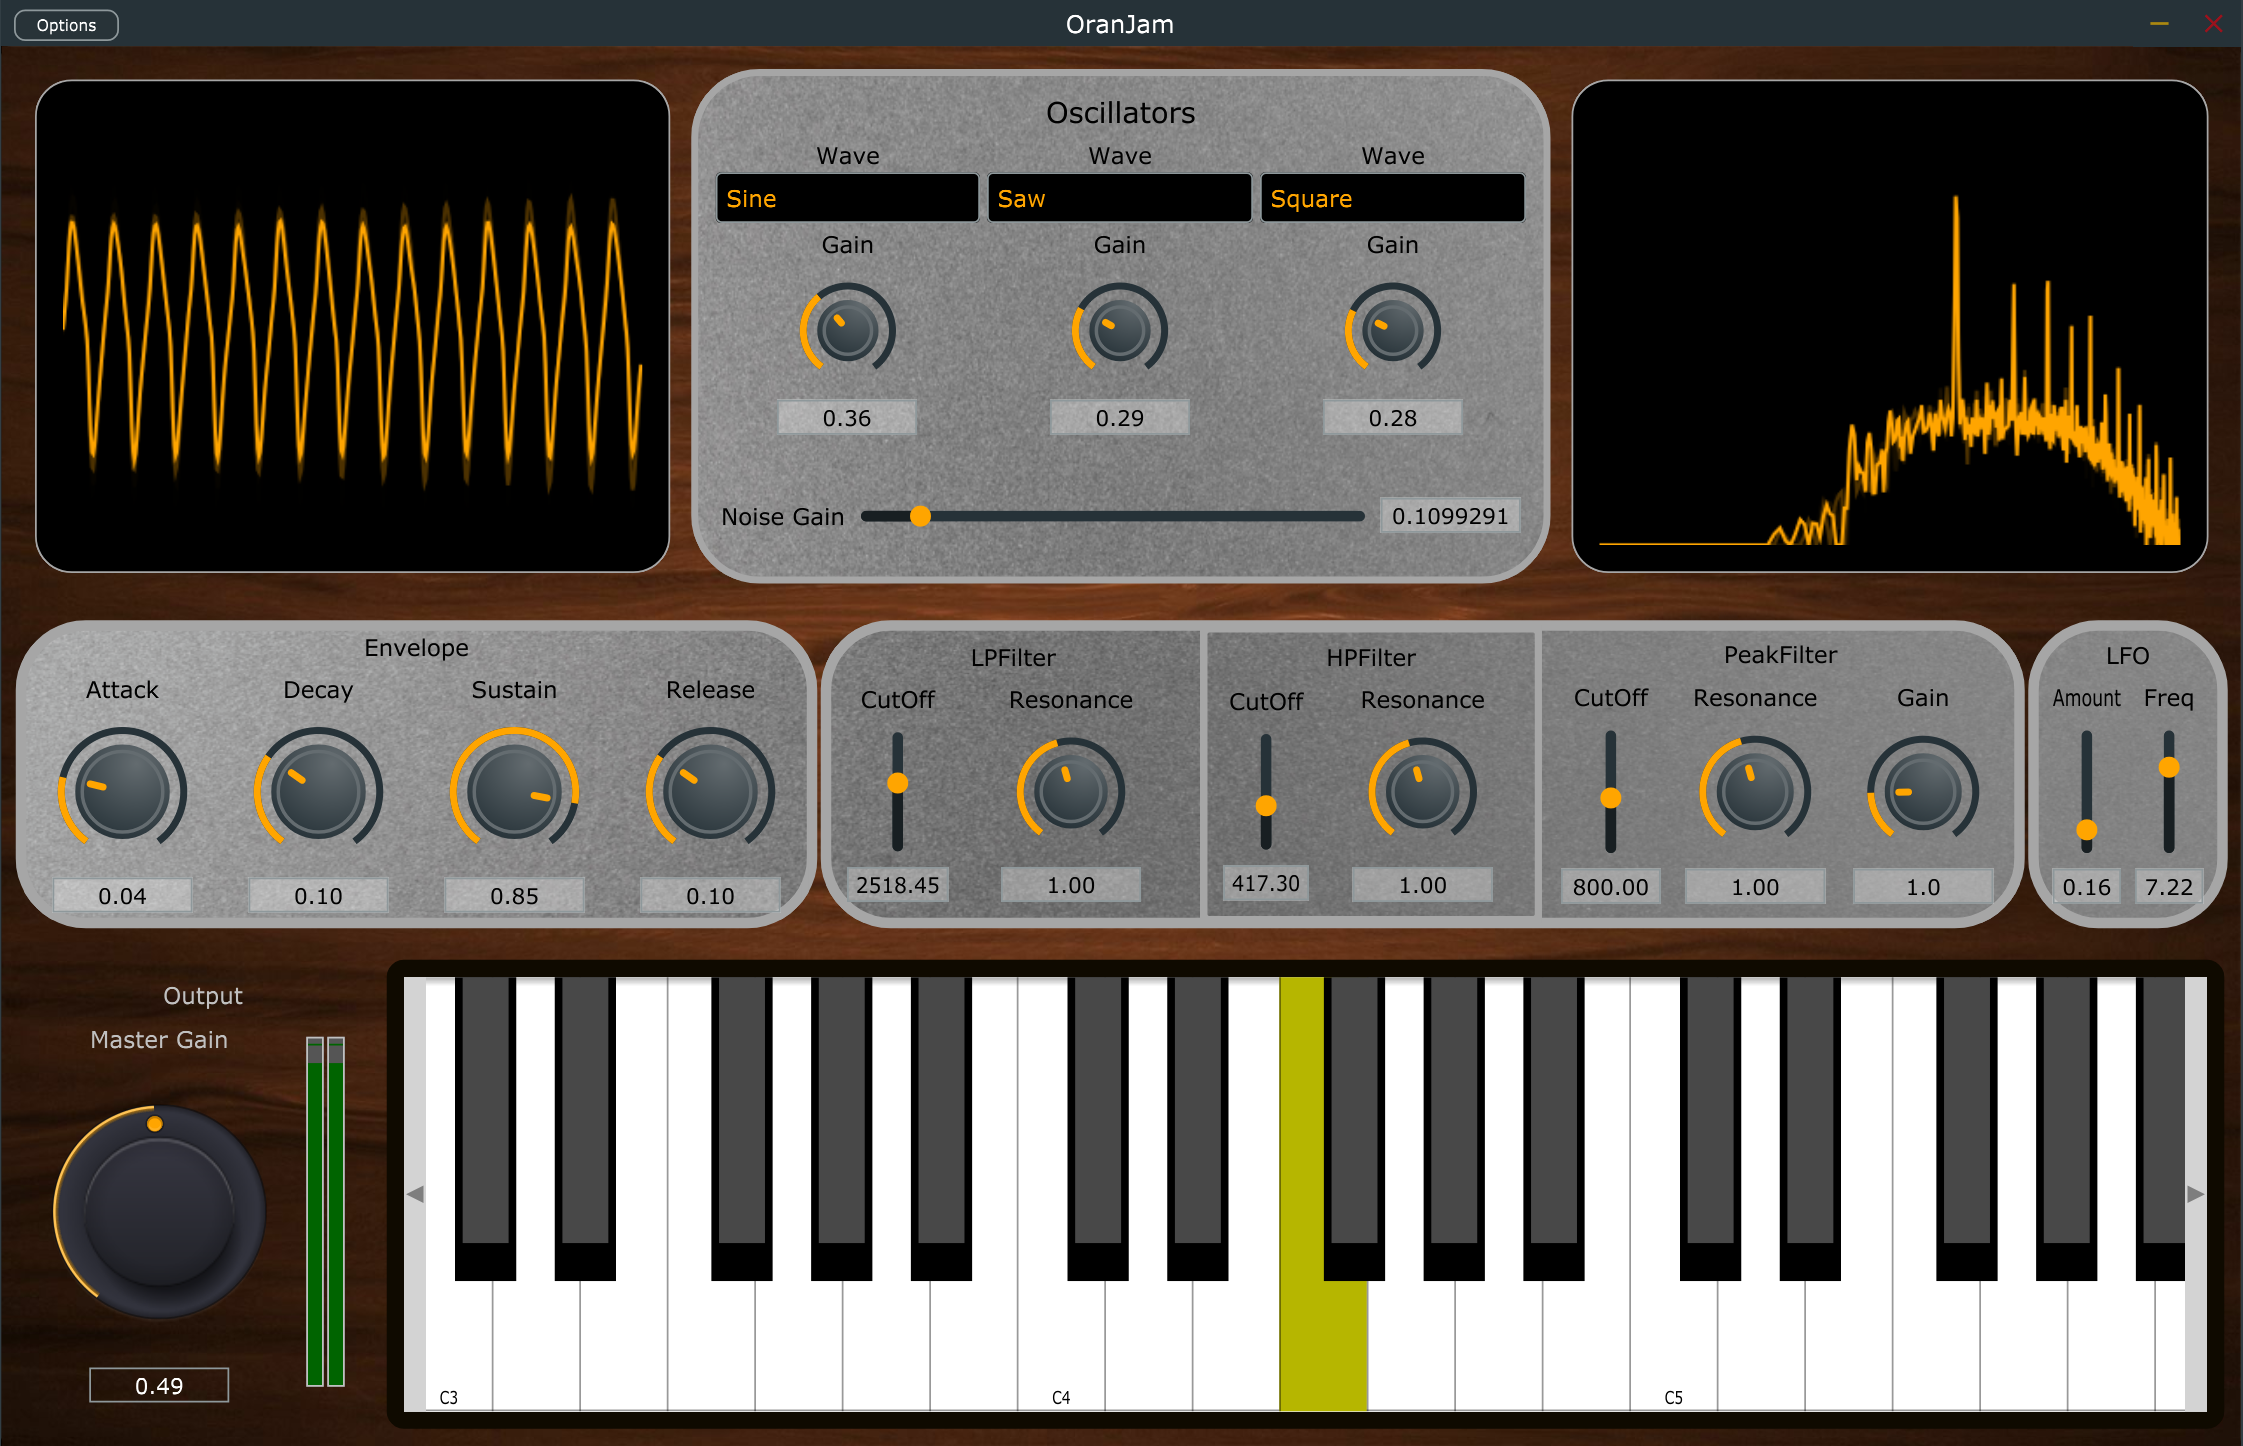
\includegraphics[width=0.75\textwidth]{DefOranJam.png}
    \caption{SubSynth Graphic User Interface}
\end{figure}
\vspace{5pt}

\subsection{Controls}
The available controls are graphically divided in six groups:

\begin{itemize}
    \item The \textbf{Keyboard} generates midi signals, allowing the user to have a ready to play virtual instrument. This is good for testing it and experimenting with it, but of course, the plugin also works with an external midi generator or an external midi keyboard, which is recommended.   \item The \textbf{Output} group, composed by\:
    \begin{itemize}
        \item The \textbf{Master Gain}, a knob at the end of the processing chain, used to control the overall output volume of the synthesizer.
        \item The \textbf{Meter}, which shows the overall output level.
   \end{itemize}
   \item The \textbf{Oscillators} group, composed by\:
    \begin{itemize}
        \item Three \textbf{Wave} selectors, one for each oscillator, that allow switching between Sinusoidal, Saw and Square waveform and the relative \textbf{Gain} knob, controlling the corresponding Volume.
        \item The \textbf{Noise Gain}, controlling the level of a random process that is added in cascade after the signal created by the oscillators and conceptually acting as an additional oscillator as well.
   \end{itemize}
   \item The \textbf{Envelope} group, composed by \textbf{Attack, Decay, Sustain} and \textbf{Release} knobs, allows the user to shape the amplitude of the played note in four moments linear regions with a linear behavior.
   \item The \textbf{Filters} group, composed by\:
       \begin{itemize}
        \item A \textbf{Low-pass Filter} that applies low-pass filtering to the signal, offering the user control on the \textbf{CutOff} frequency and \textbf{Resonance}, which boosts the signal around the frequency of \textbf{CutOff} by the selected amount.
        \item An \textbf{High-pass Filter} that applies high-pass filtering to the signal, offering the user control on the \textbf{CutOff} frequency and Resonance, which boosts the signal around the frequency of Cutoff by the selected amount. 
        \item A \textbf{Peak Filter} that applies a \textit{peak filter} to the signal, offering the user control on the \textbf{CutOff} frequency, \textbf{Gain}, which boosts the signal around the frequency of Cutoff by the selected amount following a bell-shaped function and \textbf{Resonance} which determines the said bell’s width.
   \end{itemize}
   \item The \textbf{LFO} group, that controls a Low Frequency Sinusoidal Oscillator, which modulates the volume of the three oscillators and the Noise, through the available knob control\:
   \begin{itemize}
       \item The \textbf{Amount} knob, which is the amplitude of the generated sinusoid.
        \item The \textbf{Frequency} knob, dictating the frequency of the oscillator.
   \end{itemize}
 \end{itemize}


\section{Conclusions}

\subsection{Results}

In conclusion, the result of our implementation is a versatile subtractive synthesizer able to generate a wide range of sounds and ready to be imported in a Digital Audio Workstation (DAW).
\\Software maintenance and future improvements are made possible thanks to the \textbf{modular} architecture adopted. Adding new features only requires the files of the new classes in the modules and, after calling the relative methods of initialization, updating and processing of these classes, new filters or other features can be easily added in the GUI and will be fully functional. The graphical user interface is also completely customizable both by modifying the $magic.xml$ file or with the dedicated graphic tool offered by \textit{foleys\_gui\_magic}, that can be activated straight from Projucer.

\subsection{Future Improvements}

Even if we think that the synthesizer we implemented could generate a very big variety of sounds, and for that reason we are quite satisfied with that, the audio plugin could still be expanded both on the graphics and its functionalities.
\\On the graphical user interface a more convenient filter box could be implemented, with the possibility of moving the cutoff and peak frequencies of the filters directly on the frequency domain.
\\Talking about the functionalities, a future goal is to implement an ADSR and a few more LFOs to control automatically the parameters of the filters, especially the frequency of the peak filter, which, controlled automatically, could generate many types of sounds similar to wind and instruments like oboe or flute. Also the variety of filters can be enlarged, adding for example notch filters or second order low-pass or high-pass filters, and maybe a distortion effect could be a good add. 


\end{document}

